%%%%%
%Soubor: ims.tex
%Datum: 9.12.2013
%Autor: Jan Wrona, xwrona00@stud.fit.vutbr.cz
%Projekt: Okruh 3: SHO Výrobní linka pro předmět IMS
%%%%%

\documentclass[a4paper, 12pt]{article}[9.12.2013]
  \usepackage[czech]{babel}
  \usepackage[utf8]{inputenc}
  \usepackage[T1]{fontenc}
  \usepackage[text={17cm, 24cm}, left=2cm, top=3cm]{geometry}

  \usepackage{graphicx}
  \graphicspath{ {./img/} }

  \usepackage{hyperref}

\begin{document}
%%%%%
%Soubor: title.tex
%Datum: 9.12.2013
%Autor: Jan Wrona, xwrona00@stud.fit.vutbr.cz
%Projekt: Okruh 3: SHO Výrobní linka pro předmět IMS
%%%%%
\begin{titlepage}
\begin{center}
\textsc{{\LARGE Vysoké učení technické v Brně}\\
\smallskip
{\Large Fakulta informačních technologií}}\\
\vspace{\stretch{0.382}}
{\LARGE Modelování a simulace}\\
\medskip
{\Huge Okruh 3: SHO Výrobní linka}\\
\vspace{\stretch{0.618}}
\end{center}
{\Large Jan Wrona \hfill \today}\\
{\Large Petr Kubinec}
\end{titlepage}

%\tableofcontents
%\clearpage

%%%%
\section{Úvod} \label{uvod}
%%%%
Úkolem tohoto projektu je sestavení simulačního modelu systému SHO výrobní
linky. Námi vybraná výrobní linka je rozvoz pizzy po Brně. Na základě simulace
s tímto modelem budeme zkoumat jednotlivé procesy při samotné výrobě. Hlavními
faktory pro zkoumání bude vytíženost pizzaře, vytíženost pizza pece a v
neposlední řadě také kapacita řidičů (aut).

Důvody tvorby simulací a experimentů v této oblasti rozhodně existují. Základem
úspěšné firmy správné a efektivní hospodaření s finančními prostředky. Cílem
experimentů tedy bude zjistit vytížení jednotlivých prvků v systému
a případný návrh optimalizace provozu firmy s nižšími náklady.

Požadovaná kritéria firmy byla tato:
\begin{itemize}
\item průměrná vytíženost pizzaře >= 60\%
\item počet řidičů a aut která mají být k dispozici, aby výtěžnost byla >= 70\%
\end{itemize}

\subsection{Zdroje faktů} \label{uvod:zdroje}
Pro získání přesných vstupních dat jsme využili osobní konzultace s majitelem
firmy Pizza-Taxi panem Ing. Vladimírem Pálenským, který nám poskytl veškerá
přesná data za účelem samotné optimalizace provozu firmy. Bral tento náš
projekt jako přínos pro firmu, kterou provozuje. Dalším našim zdrojem informací
bylo kontaktování gastro firem, abychom zjistili přesná čísla o poruchovosti
zařízení (v našem případě pizza pece).

Hlavní parametry pro zkoumání firmy:
\begin{itemize}
    \item jeden pizzař
    \item jedna pizza pec pro čtyři kusy pizz
    \item tři řidiči každý den (12,5 hodiny)
\end{itemize}

Zkoumaná firma má otevírací dobu od 10:30 do 23:00. V celkové otevírací době
12:30 se vyskytují 2 specifické časové oblasti s jinou střední hodnotou, které
budou při experimentech nejzajímavější:
\begin{enumerate}
    \item obědy (11:30 – 13:00)
    \item večeře (18:00 – 21:00)
\end{enumerate}
Zbytek otevírací doby je běžný provoz.

Dle informací od majitele firmy zákazníci neradi dlouho čekají na svou
obědnávku, proto pokud se nahromadí větší množství objednávek v
systému, doby čekání ve frontách se prodlužují je tak běžné že zákazník do 2
hodin od obědnání volá a obědnávku ruší.
\subsection{Validita modelu} \label{uvod:validita}
Při vytváření modelu jsme čerpali z výše uvedených zdrojů. Námi vytvořený model
se chová dle očekávaní majitele firmy a odpovídá reálnému běhu firmy.

%%%%
\section{Rozbor tématu a použitých metod/technologií} \label{rozbor}
%%%%
Modelovaná firma (výroba a rozvoz pizzy) se dá rozložit do 4 významných částí.
Jsou jimi:
\begin{enumerate}
    \item příjem objednávek
    \item příprava těsta a zdobení pizzy
    \item pečení pizzy
    \item expedice
\end{enumerate}
Každá z těchto částí pro nás znamenala zkoumání a zjišťování faktů jak už
osobním pozorováním nebo konzultací s majitelem firmy. V počátečním návrhu
jsme nepředpokládali takové množství problémů, možností a stavů které
můžou nastat.

Ad 1.: tato část v sobě zahrnuje příjem objednávek a přiřazování prioriy.
Námi zkoumaná firma dostává objednávky od 3 zdrojů:
\begin{itemize}
\item firemní objednávky
\item bowling
\item ostatní
\end{itemize}

Když se podíváme na procentuální rozdělení (tabulka \ref{tab:objednavky}), tak firemní objednávky
tvoří 8\% celkových objednávek, bowling 12\% a ostatní zbývajících 80\%. Jsou to
čísla braná ze statistiky za poslední 3 měsíce a zaokrouhlená na celé číslo. Na
první pohled se může zdát, že 8\% je nízké číslo. Ale opak je pravdou. Právě na
tyto firemní objednávky je kladen největší důraz a mají nejvyšší prioritu. Je
to vše zapříčiněno tím, že firemní objednávky nechodí často, ale ve větším
počtu. Naopak ostatní objednávky jsou procentuálně na vysoké úrovni, ale bývají
to objednávky po jednom kuse. Druhou skupinou je bowling, ten má vyšší prioritu
než ostatní objednávky, protože jsou firmy dohodnuté na jiných podmínkách
(čas doručení do 60-ti minut).

\begin{table}[h]
\centering
\begin{tabular}{ c | c | c }
    Skupina & počet objednavek/měsíc (říjen) & procentuální vyjádření\\
    \hline
    firemní objednávky & 384 & 8\%\\
    bowling	& 576 & 12\%\\
    ostatní	& 3840 & 80\%\\
    \hline
    celkem & 4800 & 100\%
\end{tabular}
\caption{Počet objednávek za měsíc}
\label {tab:objednavky}
\end{table}

Ad 2.: námi zkoumaná firma má zavedený systém, že pizzař si z jednotlivých
objednávek vytváří dávky. Tyto dávky mohou obsahovat maximálně 4ks, což je
kapacita jednoho patra v pizza peci. Samozřejmě pokud pizzař je zrovna volný a
už se mu nakumulovalo i méně než 4ks pizz (tzn. 3, 2 nebo 1ks), začne vytvářet
dávku s menším množstvím. Je tím pádem menší vytíženost pece, ale objednávky
rychleji postupují směrem k expedici. Zde je třeba uvést čas, který stráví
pizzař přípravou jedné pizzy ve várce. Tento čas se pohybuje v rozmezí 4 až 5
minut, záleží na náročnosti a složení pizzy.

Ad 3.: tento proces je velice jednoduchý, spočívá pouze v přesunutí várky do
pizza pece. Zde se tato várka peče určitou dobu. Stojí zde snad za zmínku
možnost vytvoření zmetku. Procentuálně se tato chyba dá vyjádřit 1\% z celkového
počtu objednávek.  Samotný proces pečení trvá po dobu 5-ti minut jedné várky. A
to bez ohledu, kolik samotná várka obsahuje pizz.

Ad 4.: proces expedice lze rozdělit na 3 lokality, kam firma dováží. Pokud to
vezmeme jednodušší formou, tak 1. zóna obsahuje Brno město. 2. zóna se nachází v
okrajových částech Brna (Bohunice, Líšeň, \dots). A poslední 3. zóna je většinou
mimo město (Modřice, Jehnice. Bílovice nad Svitavou, \dots) Do jednotlivých zón
je čas stráveným řidičem k doručení objednávky odlišný (tabulka \ref{tab:rozvoz}). V našem
modelu jsme neměli potřebu zavádět tento odlišné časy doručení. Vypočítali jsme
si proto průměr doručení s odchylkou, o kterou může být čas nižší nebo vyšší.

\begin{table}[h]
\centering
\begin{tabular}{ c | c | c | c}
    SZóna & počet objednavek/měsíc (říjen) & průměrný čas (min) & procentuální vyjádření\\
    \hline
    1. & 2500 & 11 & 52\%\\
    2. & 1500 & 18 & 31\%\\
    3. & 800 &  22 & 17\%\\
    \hline
    celkem & 4800 & 15 & 100\%
\end{tabular}
\caption{Doba rozvozu}
\label {tab:rozvoz}
\end{table}

Nesmíme opomenout zmínit závody zařízení (v našem případě pizza pec), které nám
poskytly gastro firmy (opravny). Samotná čísla nás trochu zaskočily, jelikož
četnost poruch těch zařízení se pohybuje průměrně kolem jedné opravy za 3
měsíce. Oprava této závady nezabere více než 2 hodiny. Dle zjištěných faktů
jasně vyplývá, že nejčastěji se jedná o poruchu v přívodním kabelu k topným
tělesům.

\subsection{Použité postupy} \label{rozbor:postupy}
Pro vytvoření našeho modelu firmy jsme využili knihovny SIMLIB/C++. Jedná se o
objektově orientovanou knihovnu pro jazyk C++. Tato knihovna patři mezi
základní nástroje pro simulaci.
\subsection{Původ použitých metod/technologií} \label{rozbor:metody}
Veškeré technologie, které jsme použili v tomto projektu byly získány z
předmětu Modelování a simulace, z dokumentace a příkladů knihovny SIMLIB/C++.

%%%%
\section{Koncepce} \label{koncepce}
%%%%
V konceptuálním návrhu dochází k zanedbání následujících vlivů, které
nejsou pro validitu systému důležíté nebo nejsou předmětem simulace:
\begin{itemize}
\item doba přijetí/zrušení objednávy: doba příjmu objednávky je tak krátká,
že by ani při nejkratším intervaleu mezi objednávkami, který se v systému může
vyskytovat, zbytek systému toto čekání nijak nemohlo ovlivnit
\item příchody objednávek na jeden kusu výrobku: model bude fungovat stejně ať už
se vygeneruje objednávka na x kusů výrobku s intervalem mezi objednávkami t
nebo x objednávek s intervaly t/x
\item rozvoz více výrobků (pizz) na stejnou adresu: ačkoli
doručení plné várky na jednu adresu bude trvat podstatně kratší dobu než
doručení plné várky na čtyři odlišné adresy, není toto třeba modelovat, protože
data o dobách rozvozů jsou zprůměrovaná na jednu pizzu
\item úrazy na pracovišti, změna pracovní směny
\end{itemize}

\subsection{Konceptuální model} \label{koncepce:model}
Popis příchodu objednávky: Nové objednávky přicházejí do bloku pro zpracování objednávek v intervalech
daných exponenciálním rozložením hustoty pravděpodobnosti se střední hodnotou
závislou na aktuální denní době. Nejčastěji objednávky
přicházeji v době večeří naopak v zavírací době nepřicházejí žádné objednávky.

Popis procesu objednávky: Objednávka je přiřazena rovnoměrným rozložením hustoty pravděpodobnosti do
jedné ze tří skupin. Rozděluje se dle poměru uvedeném v sekci \ref{rozbor}
na firemní s největší prioritou, bowlingové s nižší prioritou a všechny ostatní
objednávky s defaultní prioritou. Každá objednávka je modelována jako
netrpělivá a odchází (je zrušena zákazníkem) po době dané vzorcem
(maximální\_čekací\_doboa - exp(1/5)), kde maximální čekací doba je 120 minut
(\ref{rozbor}). Objednávka se pokusí obsadit zařízení pizzař. Pokud
rařízení není volné, zařádí se do prioritní frotny na pořadí odpovídající své
prioritě a době příchodu. Pokud pizzař je volný, proces objednávky jej obsadí.
Obsazení tohoto zařízení spustí vytvoření nové várky, objednávka tedy slouží
jako trigger.

Tvorba nové várky: Je vytvořena instance várky a proces
objednávky, který momentálně obsazuje zařízení pizzař (trigger) je do této
várky vložen. Následně jsou do várky vkládány objednávky z vrcholu
fronty před pizzařem tak dlouho, dokud není zmiňovaná fronta prázdná anebo
dokud není várka plná. Ačkoli trigger objednávka je již vložena do várky,
v kódu pokračuje dále kde vloží vytvořenou várku do fronty před pizzaře.
Várka musí mít nejvyšší prioritu, protože je ve frontě nutné ji zařadit na
první místo. Trigger proces objednávky následně uvolňuje zařízení pizzař a
pozastaví svůj běh na neurčito\footnote{Slide 172}. Uvolněním zařízení se do
zařízení dostala várka tímto procesem vytovřena, protože byla na vrcholu
fronty díky své nejvyšší prioritě. V tomto okamžiku je vytvořen objekt
zapouzdřující 1-n objednávek, který obsazuje pizzaře.

Popis procesu várky: Vysoká priorita várky již dále není potřeba, proto je tomuto procesu nastavena
defaultní priorita.

Příprava: Várka vchází do části systému, který simuluje přípravu těsta a jeho zdobení
surovinami. Doba trvání tohoto úkonu je 4 - 5 minut
rovnoměrně pro každý výrobek ve várce. Kvůli netrpělivým objednávkám není
možné spočítat počet objednávek ve várce a tolikrát čekat, je třeba zvolit
jiný přístup, protože může nastat situace, kdy při přípravě prvního výrobku ve
várce vyprší ostatním časovač a odejdou ze systému. Validita by potom utrpěla
na přípravě už zrušených objednávek. Řešením je v každé iteraci kontrolovat,
zda se daná objednávka ve várce ještě skutečně vyskytuje a dle toho upravit
následující akce. Po zpracování všech objednávek ve várce je uvolněno zařízení
pizzař.

Kontrola zmetků: Každý výrobek po výstupu z přípravy projde kontrolou a s 1\% pravděpodobností
(\ref{rozbor}) je na výrobku nalezena nějaká chyba. Tato část neobsahuje
žádné čekání, protože kontrola je běžně prováděna současně s přípravou, zde
jsou tyto bloky odděleny z důvodu lepší přehlednosti.

Pečení: Ještě před obsazením pece je nutné zkontrolovat, zda během předchozích
čekání nevypršely všem objednávkám časovače. V takovém případě by byla várka
prázdná a pec by byla zabrána prázdnou várkou. Jednoduchou podmínkou se tomu
lze vyhnout. Várka se potom pokouší o obsazení pizza pece. Zde bych zdůraznil,
že všem várkám byla dříve nastavena výchozí hodnota priority. Ve várce se již
nerozlišuje zda všechny její objednávky mají vysokou prioritu či naopak. Tento
koncept je totožný se zacházením s objednávkami v modelovaném systému, kde se
prioritní fronty tvoří pouze před přípravou pizzy. Při volné peci proběhne
pečení s přesnou dobou trvání pět minut (\ref{rozbor}) bez ohledu na počet
výrobků ve várce. Po uplynutí této doby je zařízení uvolněno a tak jako u
přípravy i zde se provádí kontrola zmetků s tím rozdílem, že se kontrolou
projdou buď všechny výrobky ve várce nebo žádný. Taková chování simuluje
především přehřátí trouby, která způsobí spálení ne konkrétních výrobků ale
všech najednou.

Doručení: Doručování se tak jako pečení nekoná, pokud je várka prázdná. Várka se pokusí
vstoupit do skladu, která zde modeluje doručovací auto s řidičem. Počet
nasazených řidičů se mění, nicméně nejčastěji mají směnu tři řidiči
proto má sklad defaultně kapacitu tři. Po vstupu do skladu (naložení várky do auta)
je proveden rozvoz o době trvání 10 až 20 minut rovnoměrně (\ref{tab:rozvoz}). I zde
stále objednávky mají běžící časovač simulující zrušení objednávky zákazníkem
po určité době, řešení této situace je totožné jako při přípravě těsta a
zdobení. Po uplynutí doby rozvozu se auto vrací zpět a várka opouští sklad.
Tímto je simulace jedné várky a jí přislušejících objednaných produktů u
konce. Úspěšně ukončeným procesům je nutné smazat časovač, především jeho
záznam v kalendáři. Neúspěšné procesy (zmetky) mají časovač již odstraněný.
Úspěšné ale i nedokončené objednávky v tomto bodě odcházejí ze systému.

\subsection{Petriho síť} \label{koncepce:ps}

\begin{figure}[h]
    \centering
    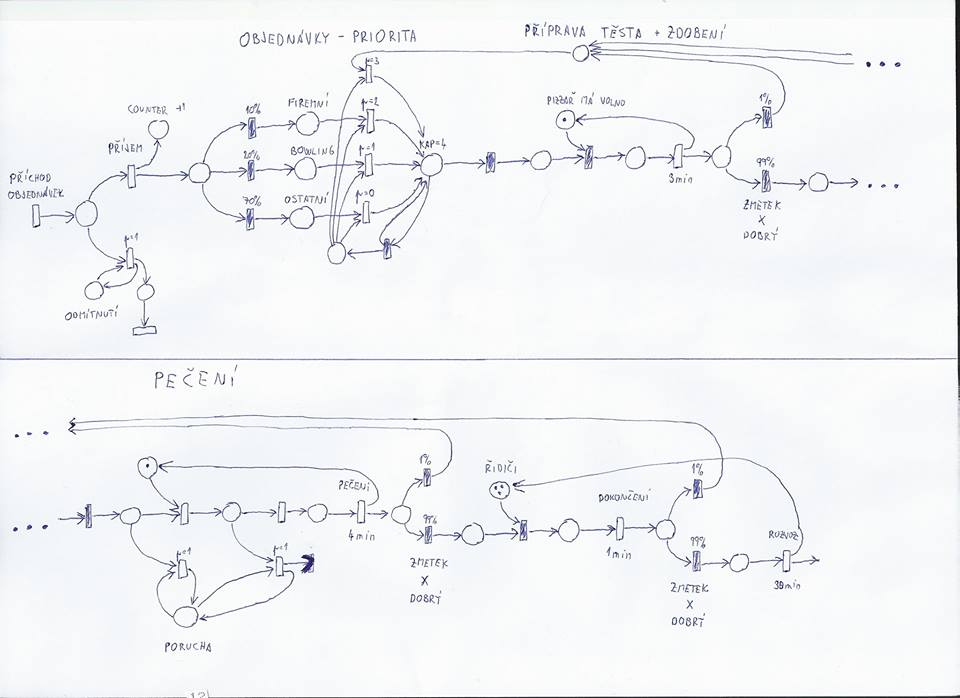
\includegraphics[width=\textwidth,height=\textheight,keepaspectratio]{ps.jpg}
    \caption{Petriho síť}
    \label{fig:petriho_sit}
\end{figure}

%%%%
\section{Architektura simulačního modelu/simulátoru} \label{architektura}
%%%%
Jedná se o simulační model vytvořený jako aplikace bez dynamických vstupů
(parametrů), veškerá data se mění ve zdrojových souborech. Výstupem je textový soubor,
ve kterém se nachází základní statistiky všech použitých zařízení, skladů a
jejich příslušných front. Překlad i spuštění je zajištěn utilitou Make a
ovládá se příkazy make, make run, make clean.

\subsection{Mapování abstraktního modelu do simulačního} \label{architektura:mapovani}
Změna denních dob je implementováno ve třídě Daytime, která dědí od třídy
Event. V její metodě Behavior() je aktivována instance třídy Generator pro
vytváření vstupních zakázek/objednávek. Objednávka je abstrahována třídou Order s rodičovskou třídou Process.
Dávka či várka, která zajišťuje zapouzdření objednávek do jednoho objektu, je
realizována třídou Batch taktéž dědící od Process. Další třída Timeout
implementuje objednávkám netrpělivost. Posledními třídami jsou FailureEvent a
FailureProcess (název napovídá jejich předky), které zajišťují vygenerování a
obsluhu (opravu) poruchy.

Všechny fronty jsou typu FIFO implementovány jako instance třídy Queue, zařízení jsou instance třídy
Facility a sklad je pro změnu instance třídy Store.


%%%%
\section{Podstata simulačních experimentů a jejich průběh} \label{experimenty}
%%%%
Cílem experimentů je optimalizace provozu firmy s nižšími náklady, nebo naopak,
jak navýšit prodej a tím pádem zvýšit zisk firmy. Budeme zjišťovat, jaké zdroje
je potřeba navyšovat, případně v určitých hodinách snižovat. Zda se nevyplatí
na určité hodiny spustit do provozu druhou pec na pizzu.

\subsection{Postup experimentování} \label{experimenty:postup}
Simulace bude probíhat následujícím způsobem. Nejdříve jsme nastavili veškeré
vstupní údaje (příjem objednávek, počet pizzařů, výtěžnost pece a kapacitu
řidičů). Zjistíme, kde se tvoří velké fronty nebo naopak, kde vznikají volná
místa (nízká využitelnost). Následně budeme jednotlivé tyto hodnoty upravovat
(navyšovat nebo ubírat), dokud nenalezneme optimální hodnoty, které pomohou ke
zlepšení firmy.

\subsection{Dokumentace experimentů} \label{experimenty:dokumentace}
Nejprve jsme provedli simulaci celého dne, abychom viděli rozložení objednávek
během dny, musíme totiž zkoumat, zda se jedná o obědy, večeře nebo období mezi
těmito úseky. Vše je znázorněno v grafu \ref{fig:1}.

\begin{figure}[h]
    \centering
    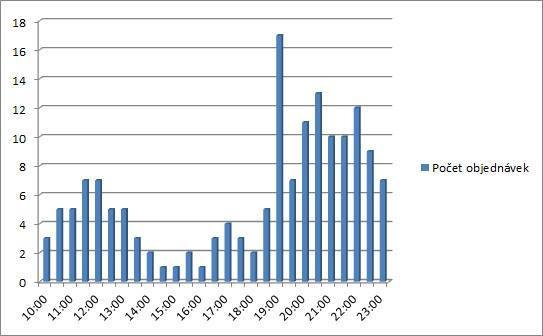
\includegraphics[width=\textwidth,height=\textheight,keepaspectratio]{1.jpg}
    \caption{Počet objednávek}
    \label{fig:1}
\end{figure}

Z grafu je patrné, že nás bude nejvíce zajímat večerní období, kdy je četnost
objednávek nejvyšší. A zároveň bude nutnost provést mnoho experimentů na
odpolední období, kdy zase nastává druhý extrém a to ten, že bude možnost
redukování počtu řidičů. Nesmíme však zapomenout i na experimenty v obědovém
období.

Za zmínku dále stojí čas, po kterou byly jednotlivé objednávky rozdělené dle
priorit na provozně, než se dostaly k expedici. Vše je zobrazeno v tabulce \ref{tab:doba}

\begin{table}[h]
\centering
\begin{tabular}{ c | c }
    Priorita & průměrný čas v systému (min)\\
    \hline
    firemní (2) & 19.8\%\\
    bowling (1) & 28.1\%\\
    ostatní (0) & 38.3\%\\
\end{tabular}
\caption{Doba rozvozu}
\label {tab:doba}
\end{table}

Důležitých faktorech pro zkoumání běhu firmy je pozorování počtu pizz v
jednotlivých dávkách. Odvíjí se od toho mnoho faktorů. Například pokud by byla
v každé dávce pouze jedna pizza, efektivnost a výtěžnost celého systému by byla
příliš nízká. Porovnáme-li druhou stránku věci, tak pokud by každá várka
obsahovala zase maximální možné množství pizz, ve velké většině případů by se
tvořily fronty na jednotlivých zařízení a celý model by se zahlcoval. V grafu \ref{fig:2} je znázorněn průměrný počet pizz ve várkách.

\begin{figure}[h]
    \centering
    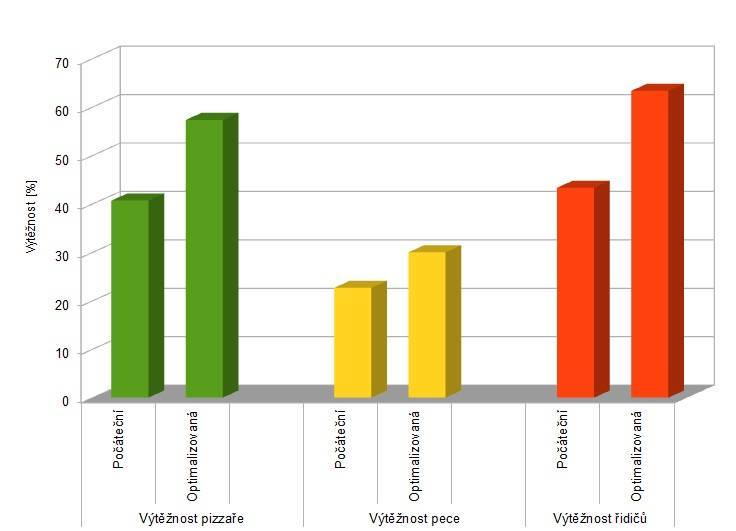
\includegraphics[width=\textwidth,height=\textheight,keepaspectratio]{2.jpg}
    \caption{Vytíženost}
    \label{fig:2}
\end{figure}

Pustíme se experimentů provozu přes obědy. Zde za aktuálních podmínek bylo
reálné využití pizzaře kolem 35\%. Fronta se nicméně vytvářela, ale malým
množstvím objednávek se vytvářely z velké části dávku o velikosti 1ks pizz a
průměrné zdržení dávky bylo 2 minuty. U čísel výtěžnosti samotné pece je jasně
patrné, že je vytěžována minimálně, cca 12\%. Fronta se zde vytvořila zhruba u
1/3 dávek. A průměrný strávený čas ve frontě byl cca 2,5 minuty. A poslední
námi zkoumaná část jsou řidiči. Z počátečního nastavení 3 řidičů je průměrná
výtěžnost lehce nad 30\%. Je tedy jasně patrné, ze v tomto období se nesplňují
optimální podmínky firmy. A to jak výtěžnost pizzaře, tak ani řidičů (aut).

Pro zlepšení podmínek jsme provedli experimenty a k optimalizaci vedla pouze
úprava počtu řidičů a to zredukováním na 2 řidiče. Nyní se výtěžnost řidičů
zvedla před 60\% a zároveň se stále netvořily velké fronty, pouze u 1/3 dávek s
průměrnou čekací dobou pod 10 minut, což splňuje podmínky firmy. A díky
experimentům můžeme firmě doporučit, aby při dvou řidičích se pokusila a
navýšení objednávek přes obědy o 20\%, pak budou splněny veškeré vstupní
podmínky.

Dále se pustíme zkoumání provozu v odpoledních hodinách (13:00 – 18:00). Nyní
se nacházíme u výtěžnosti pizzaře pod 27\%, fronta byla takřka nulová. A většina
dávek obsahovala jednu pizzu a maximálně dva kusy pizz s tím, že zdržení dávek
bylo průměrně lehce pod 1 minutu. Pizza pec má stejnou výtěžnost jako v
poledních hodinách. Sice se dělá menší množství objednávek, nicméně počet dávek
je zhruba stejný. Proto je výtěžnost stejná, ale mnohem nižší využití. Pokud je
již vytvořila fronta u pizza pece (cca 10\%), byla průměrná doba strávená ve
frontě pod 1 minutu. U počátečního stavu 3 řidičů byla výtěžnost pod 20\%
procent a fronta se vytvářela zhruba u 1/4 objednávek, s průměrným časem 4,2
minuty.

Experimenty prováděné v tomto období byly opět směřované především na
počet řidičů. Zde již nebylo nalezeno jednoznačného řešení. Nastaly zde 2
možnosti řešení k nalezení lepšího řešení. Jednou je možnost opět omezení
řidičů na 2. Dostaneme se pak k výtěžnosti řidičů přes 50\% a fronty se
vytvářejí u 1/3 dávek s průměrnou dobou 4,5 minut. Nebo je pak možnost omezit
řidiče na 1, zmiňovaná výtěžnost se zvedne přes 80\%, ale nastává zde problém s
čekáním dávek ve frontách. Průměrný čas se sice pohybuje kolem 25 minut, což by
ještě splňovalo podmínky firmy. Ale už byl i maximální čas 85 minut, toto číslo
již je velice špatné. Proto se opět volí jako ideální varianta opět 2 řidiči. A
aby se firma pokusila o navýšení objednávek o 100\% a bude model vytěžován
efektivně a budou splněny veškeré podmínky firmy.

Poslední částí z experimentů je večerní provoz. Zde je výtěžnost pizzaře přes
60\%. Každopádně se zde již začaly tvořit fronty dávek u pizzaře a to zhruba u
2/3 příchozím objednávek, ale průměrný čas byl 7,2 minuty. Zde většina
objednávek obsahovala 2 kusy pizz. Podíváme-li se na výtěžnost pece, dostáváme
se k číslům kolem 45\%. A už se zde hromadí i várky u poloviny objednávek s
průměrnou dobou 5 minut. U řidičů je výtěžnost při těchto požadavcích přes 80\%
a průměrnou dobou čekání 18,2 minut. Už se již zde navýšilo číslo objednávek, u
kterých vypršel timeout a byly tudíž odstraněny ze systému, stalo se tak u 2
objednávek.


V tomto období jsou splněny veškeré podmínky firmy. Provedli jsme mnoho
experimentů, za účelem navýšení efektivnosti, ale žádná z možností se neukázala
jako lepší. Byla by možnost pořídit ještě jednou pec s kapacitou 4 ks pizz, ale
mělo by to za následek zvýšení ztrátovosti objednávek, protože by se tvořily
velké fronty u řidičů.

\subsection{Závěry experimentů} \label{experimenty:zavery}
Pomocí experimentů se podařilo zjistit optimální stavy, aby byly splněny
požadovaná kritéria firmy. Pro zobrazení výsledků našich experimentů poslouží
graf \ref{fig:3} ve kterém se porovnají počáteční a námi optimalizovaná data.

\begin{figure}[h]
    \centering
    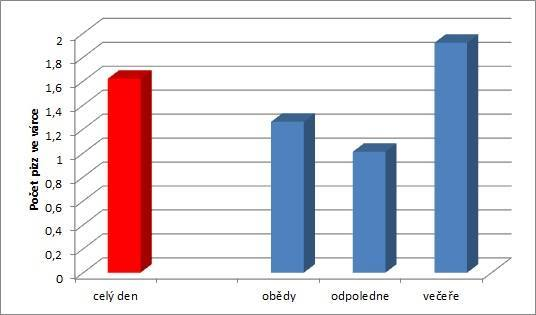
\includegraphics[width=\textwidth,height=\textheight,keepaspectratio]{3.jpg}
    \caption{Počet pizz ve várce}
    \label{fig:3}
\end{figure}

Z grafu je vidět, že jsou splněny vstupní kritéria firmy. A to výtěžnost
pizzaře je přes 50\% a výtěžnost řidičů je přes 60\%.
\clearpage
%%%%
\section{Shrnutí simulačních experimentů a závěr} \label{zaver}
%%%%
V rámci projektu do předmětu IMS byl sestaven simulační model SHO výrobní
linky. Na základě experimentů bylo určeno optimální nastavení systému pro
efektivní výtěžnost firmy za splňujících kritérií. Veškeré výsledné nastavení
je uvedeno v tabulce.  Dále bylo experimenty zjištěno, o kolik by firma musela
navýšit příjem objednávek v určitém období dne, aby byly zachovány veškeré
požadavky firmy a zároveň se zlepšila výtěžnost jednotlivých prvků v systému
dle zadaných kritérií (tabulka \ref{tab:final}).

\begin{table}[h]
\begin{tabular}{ c | c | c | c | c | c }
    Období & Počet řidičů & Výtěžnost pizzaře & Výt. pece & Výt. expedice & Navýšení obj.\\
    \hline
    obědy     & 2 & 35\% & 12\% & 60\% & 20\%\\
    odpoledne & 2 & 27\% & 11\% & 50\% & 100\%\\
    večer     & 3 & 60\% & 45\% & 80\% & 0\%
\end{tabular}
\caption{Doba rozvozu}
\label {tab:final}
\end{table}
\end{document}
